\documentclass{article}
\usepackage{titlesec}

\usepackage[citestyle=authortitle-terse,backend=bibtex]{biblatex}
\addbibresource{bibliography.bib}

\setcounter{secnumdepth}{0}
\usepackage{sectsty}
\sectionfont{\fontsize{17}{20}\selectfont}

\usepackage[left=4cm, right=4cm]{geometry}
\usepackage{palatino,eulervm,dutchcal,xcolor}%fonts
\usepackage{graphicx,subcaption,float}
\usepackage{enumitem,parskip,multicol}
\usepackage{amsthm,amssymb,amsmath,mathtools,thmtools}
\usepackage{tikz,tikz-cd}
\usetikzlibrary{%
	matrix,%
	calc,%
	arrows,%
	shapes,
	decorations.markings,backgrounds,calc,intersections}
\tikzcdset{scale cd/.style={every label/.append style={scale=#1},
		cells={nodes={scale=#1}}}}
\usepackage[bookmarks,bookmarksopen,bookmarksdepth=3]{hyperref}
\hypersetup{%colores
	colorlinks=true,
	urlcolor=blue,
	linkcolor=magenta,
	citecolor=blue,
	filecolor=blue,
	urlbordercolor=white,
	linkbordercolor=white,
	citebordercolor=white,
	filebordercolor=white}
\usepackage{cleveref}
\Crefname{exercise}{Exercise}{Exercises}

\newcommand{\fakesection}[1]{%
	\par\refstepcounter{section}% Increase section counter
	\sectionmark{#1}% Add section mark (header)
	\addcontentsline{toc}{section}{\protect\numberline{\thesection}#1}% Add section to ToC
	% Add more content here, if needed.
}

\makeatletter %Hide section number
\def\@seccntformat#1{%
	\expandafter\ifx\csname c@#1\endcsname\c@section\else
	\csname the#1\endcsname\quad
	\fi}
\makeatother

\definecolor{blue-violet}{rgb}{0.54, 0.17, 0.89}
\definecolor{azure}{rgb}{0.0, 0.5, 1.0}
\definecolor{green(ncs)}{rgb}{0.0, 0.62, 0.42}
\definecolor{forestgreen}{rgb}{0.13, 0.55, 0.13}
\definecolor{limegreen}{rgb}{0.2, 0.8, 0.2}
\definecolor{palatinateblue}{rgb}{0.15, 0.23, 0.89}
\definecolor{trueblue}{rgb}{0.0, 0.45, 0.81}
\definecolor{goldenyellow}{rgb}{1.0, 0.87, 0.0}
\definecolor{fashionfuchsia}{rgb}{0.96, 0.0, 0.63}
\definecolor{brightcerulean}{rgb}{0.11, 0.67, 0.84}
\definecolor{jonquil}{rgb}{0.98, 0.85, 0.37}
\definecolor{lavendermagenta}{rgb}{0.93, 0.51, 0.93}
\definecolor{peru}{rgb}{0.8, 0.52, 0.25}
\definecolor{persimmon}{rgb}{0.93, 0.35, 0.0}
\definecolor{persianred}{rgb}{0.8, 0.2, 0.2}
\definecolor{persianblue}{rgb}{0.11, 0.22, 0.73}
\definecolor{persiangreen}{rgb}{0.0, 0.65, 0.58}
\definecolor{persianyellow}{rgb}{0.9, 0.89, 0.0}

\declaretheoremstyle[headfont=\color{trueblue}\normalfont\bfseries,]{colored1}
\declaretheoremstyle[headfont=\color{forestgreen}\normalfont\bfseries,]{colored2}
\declaretheoremstyle[headfont=\color{peru}\normalfont\bfseries,]{colored3}
\declaretheoremstyle[headfont=\color{persiangreen}\normalfont\bfseries,]{colored4}
\declaretheoremstyle[headfont=\color{brightcerulean}\normalfont\bfseries,]{colored5}
\declaretheoremstyle[headfont=\color{lavendermagenta}\normalfont\bfseries,]{colored6}
\declaretheoremstyle[headfont=\color{blue-violet}\normalfont\bfseries,]{colored7}
\declaretheoremstyle[headfont=\color{green(ncs)}\normalfont\bfseries,]{colored8}
\declaretheoremstyle[headfont=\color{peru}\normalfont\bfseries,]{colored9}
\declaretheoremstyle[headfont=\color{persiangreen}\normalfont\bfseries,]{colored10}

\declaretheorem[style=colored1,numberwithin=section,name=Theorem]{thm}
\declaretheorem[style=colored2,numberwithin=section,numberlike=thm,name=Proposition]{prop}
\declaretheorem[style=colored3,numberwithin=section,numberlike=thm,name=Lemma]{lemma}
\declaretheorem[style=colored4,numberwithin=section,numberlike=thm,name=Corollary]{coro}
\declaretheorem[style=colored5,numbered=no,name=Example]{example}
\declaretheorem[style=colored5,numbered=no,name=Examples]{exemplos}
\declaretheorem[style=colored7,numberwithin=section,name=Exercise]{exercise}
\declaretheorem[style=colored9,numbered=no,name=Remark]{remark}
\declaretheorem[style=colored9,numbered=no,name=Claim]{claim}
\declaretheorem[style=colored8,numbered=no,name=Definition]{defn}
\declaretheorem[style=colored10,numbered=no,name=Question]{question}

\newcommand{\R}{\mathbb{R}}
\newcommand{\Z}{\mathbb{Z}}
\newcommand{\N}{\mathbb{N}}
\newcommand{\C}{\mathbb{C}}
\newcommand{\Q}{\mathbb{Q}}
\newcommand{\D}{\mathbb{D}}
\newcommand{\T}{\mathbb{T}}
\renewcommand{\P}{\mathbb{P}}
\newcommand{\Ac}{\mathcal{A}}
\newcommand{\Bc}{\mathcal{B}}
\newcommand{\Cc}{\mathcal{C}}
\newcommand{\Dc}{\mathcal{D}}
\newcommand{\Ec}{\mathcal{E}}
\newcommand{\Fc}{\mathcal{F}}
\newcommand{\Gc}{\mathcal{G}}
\newcommand{\Lc}{\mathcal{L}}
\newcommand{\Oc}{\mathcal{O}}
\newcommand{\Qc}{\mathcal{Q}}
\newcommand{\Sc}{\mathcal{S}}
\newcommand{\Wc}{\mathcal{W}}
\newcommand{\mf}{\mathfrak{m}}
\newcommand{\gf}{\mathfrak{g}}
\newcommand{\X}{\mathfrak{X}}
\newcommand{\hf}{\mathfrak{h}}
\newcommand{\glf}{\mathfrak{gl}}
\newcommand{\of}{\mathfrak{o}}

\renewcommand{\Im}{\operatorname{Im}}
\renewcommand{\O}{\operatorname{O}}
\renewcommand{\S}{\mathbb{S}}
\renewcommand{\T}{\mathbb{T}}
\DeclareMathOperator{\Lie}{\operatorname{Lie}}

\DeclareMathOperator{\img}{img}
\DeclareMathOperator{\Arg}{Arg}
\DeclareMathOperator{\End}{End}
\DeclareMathOperator{\I}{I}
\DeclareMathOperator{\id}{id}
\DeclareMathOperator{\Id}{Id}
\DeclareMathOperator{\Alt}{Alt}
\DeclareMathOperator{\sgn}{sgn}
\DeclareMathOperator{\supp}{supp}
\DeclareMathOperator{\Int}{Int}
\DeclareMathOperator{\Ob}{Ob}
\DeclareMathOperator{\Mor}{Mor}
\DeclareMathOperator{\Top}{Top}
\DeclareMathOperator{\CGWH}{CGWH}
\DeclareMathOperator{\Hom}{Hom}
\DeclareMathOperator{\Map}{Map}
\DeclareMathOperator{\Tot}{Tot}
\DeclareMathOperator{\Vect}{Vect}
\DeclareMathOperator{\VectBund}{VectBund}
\DeclareMathOperator{\Open}{Open}
\DeclareMathOperator{\Ring}{Ring}
\DeclareMathOperator{\Set}{Set}
\DeclareMathOperator{\GL}{GL}
\DeclareMathOperator{\SL}{SL}
\DeclareMathOperator{\SO}{SO}
\DeclareMathOperator{\U}{U}
\DeclareMathOperator{\SU}{SU}
\DeclareMathOperator{\Sp}{Sp}
\DeclareMathOperator{\M}{M}
\DeclareMathOperator{\Aut}{Aut}
\DeclareMathOperator{\PGL}{PGL}
\DeclareMathOperator{\PSL}{PSL}
\DeclareMathOperator{\St}{St}
\DeclareMathOperator{\Vol}{Vol}

\begin{document}
\begin{minipage}{\textwidth}
	\begin{minipage}{.5\textwidth}
		Complex Manifolds in Dimension 1\\
	\end{minipage}%
	\begin{minipage}{.5\textwidth}
		\raggedleft
		Daniel González Casanova Azuela\par
		{\small\href{https://github.com/danimalabares/riemann-surfaces}{github.com/danimalabares/riemann-surfaces}}
	\end{minipage}%
\end{minipage}\vspace{.2cm}\hrule
\section{Home Assignment 4: Orientations}
\setcounter{section}{4}
\begin{defn}
	\textbf{\textit{Determinant bundle}} on an $n$-dimensional smooth manifold is the bundle $\Lambda^n(M)$ of antisymmetric $n$-linear forms. A manifold is called \textbf{\textit{orientable}} if its determinant bundle is trivial.
\end{defn}

\begin{remark}
	A real line bundle is trivial if and only if it admits a nowhere-vanishing section.
\end{remark}

\begin{defn}
	If $M$ is an orientable manifold, a map $f:M\to M$ is \textbf{\textit{orientation preserving}} if there is a nowhere-zero section $\omega$ of $\Lambda^n(Y)$ such that $f^*\omega$ has the opposite sign.
\end{defn}

\begin{exercise}
	Let $S$ be a compact Riemann surface. Prove that there exists a free action of the group $\Z/2$ on $S$ reverting the orientation.
	\begin{enumerate}[label=\alph*.]
		\item When $S$ is a torus or a sphere. 
		\item When the genus of $S$ is even.
		\item When the genus of $S$ is odd.
	\end{enumerate}
\end{exercise}
\begin{proof}[Solution]\leavevmode
		Any reflection inverts orientation, and the composition of an odd number of reflections reverts orientation. The map $-\Id:S^2\to S^2$ reverts orientation because is the composition of 3 reflections.
		
		\textit{Idea:} the restriction of $-\Id$ to any Riemann surface embedded in $\R^3$ ``symmetrically" about the origin is the map we are looking for.
\end{proof}

\begin{exercise}
	 Let $M$ be an almost complex manifold. Prove that it is
	orientable.
\end{exercise}
\begin{proof}
	(From \href{https://math.stackexchange.com/questions/1817959/almost-complex-manifolds-are-orientable}{StackExchange}.) We have seen that given any Riemannian metric $g$ on $M$, the metric $h=g+I(g)$ is hermitian, that is, $I$-invariant. Also, the bilinear form $\omega(x,y):=g(x,Iy)$ is skew-symmetric and non-degenerate. The latter follows from the identity $\omega(x,-)=-h(Ix,-)$ and the fact that $h$ is non-degenerate since $g$ is non-degenerate. Then $\omega$ is an element of $\Lambda^1(M)$, and $\omega\wedge\ldots\wedge\omega$ an element of $\Lambda^n(M)$ that does not vanish.
\end{proof}
\begin{exercise}
	Let $S \subset \R^3$ be a smooth compact 2-dimensional submanifold of $\R^3$. Prove that it is orientable.
\end{exercise}
\begin{proof}[Solution]
	%I couldn't directly construct a nowhere vanishing section of $\Lambda^2(S)$. So I looked in \cite{lee} and found that it suffices to find a smooth unit normal vector field along $S$ (prop. 15.32). But how? Specially considering the case of the Möbius strip, for which such a vector field should not exist.
	
	The Jordan-Bruower Separation Theorem states that the complement of a compact, connected hypersurface $S$ in $\R^n$ consists of two connected open sets, the "outside" $D_0$ and the "inside"  $D_1$. Moreover, $\overline{D_1}$ is a compact manifold whose boundary is $S$ (p. 89 \cite{guillemin}).
	
	For any Riemannian manifold with boundary such as $\overline{D_1}$ there is a unique smooth outward-pointing unit vector $N$ field along its boundary (prop. 15.33 \cite{lee}). In turn, this means that the form 
	\[N\lrcorner\Vol_{\R^3}=\iota_N\Vol_{\R^3}\in\Lambda^2(\partial\overline{D_1})=\Lambda^2(S)\]
	does not vanish.
\end{proof}
\begin{exercise}
	Let $M$ be a manifold with fundamental group isomorphic to $\Q$. Prove that $M$ is orientable.
\end{exercise}
\begin{proof}[Solution]
	Suppose $M$ is connected. Let $\tilde{M}$ be the orientable two-sheeted covering space of $M$. Recall that the number of sheets of a covering space $p:(\tilde{M},\tilde{x}_0)\to(M,x_0)$ equals the index of $p_*(\pi_1(\tilde{X},\tilde{x}_0))$ in $\pi_1(M,x_0)$ provided both $M$ and $\tilde{M}$ are path connected. $\Q$ has no subgroups of index 2, so $\tilde{M}$ cannot be connected (prop. 1.32, \cite{hatcher}). Then $\tilde{M}$ must have two connected components since it is a two-sheeted covering space of a connected manifold. Each of the two connected components of $\tilde{M}$ is homeomorphic to $M$, and since $\tilde{M}$ is orientable so is $M$.
\end{proof}
\begin{figure}[H]
	\centering
	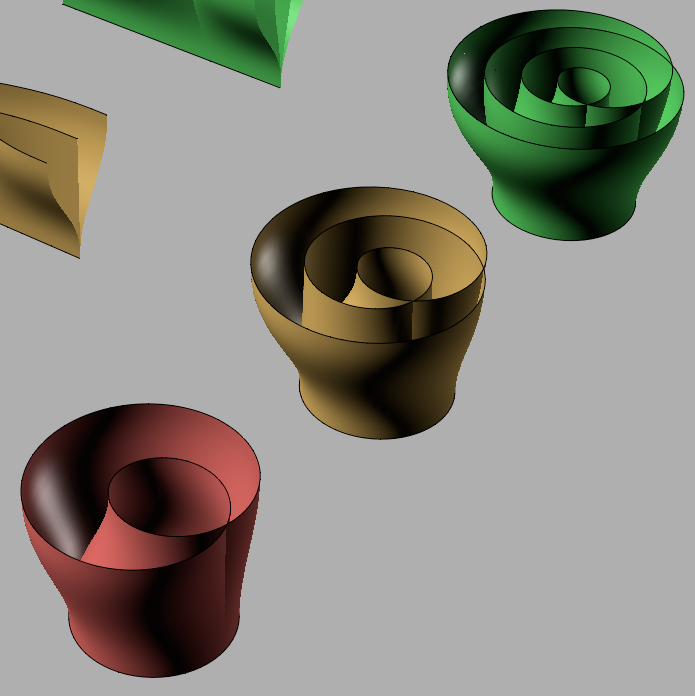
\includegraphics[width=0.355\linewidth]{rational-circle1}\hspace{2cm}
	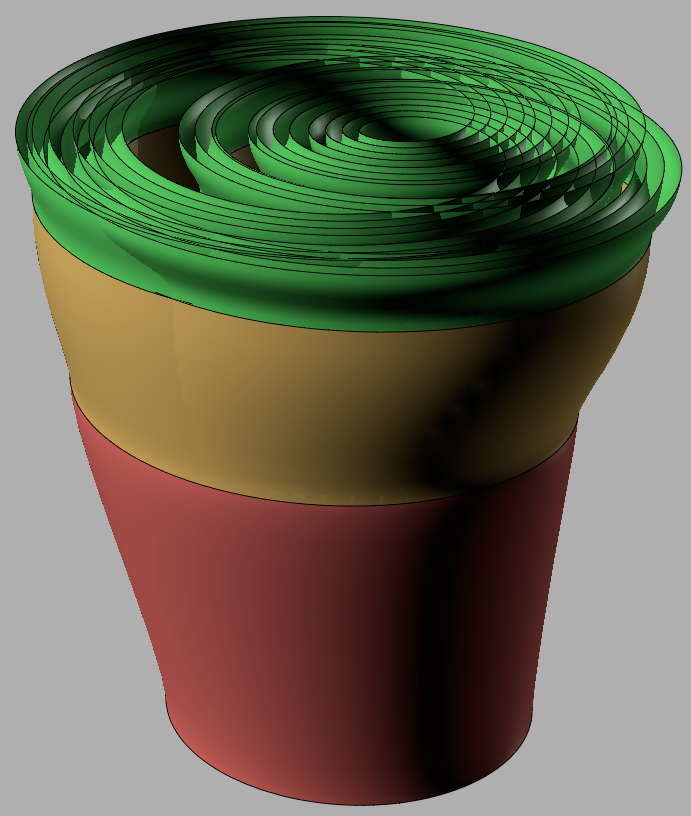
\includegraphics[width=0.3\linewidth]{rational-circle2}
	\caption*{\textit{Gluing cylinders to construct the \textbf{\textit{rational circle}}, a space with fundamental group $\Q$. (\cite{rational-circle})}}
\end{figure}

\begin{exercise}
	Let $G$ be a Lie group. Prove that its fundamental group is commutative.
\end{exercise}
\begin{proof}[Solution]
	A standard argument found in \href{https://math.stackexchange.com/questions/727999/g-is-topological-implies-pi-1g-e-is-abelian}{StackExchange} uses the Eckmann–Hilton argument as follows. We show that the operation
	\begin{align*}
		*:\pi_1(G)\times\pi_1(G)\cong\pi_1(G\times G)&\longrightarrow\pi_1(G)\\\\
		([f],[g])\qquad\qquad&\mapsto[fg]
	\end{align*}
	satisfies the following relation with respect to the usual product $\cdot$ on $\pi_1(G)$:
	\begin{equation}\label{eq:eck}
		(a*b)\cdot(c*d)=(a\cdot c)*(b\cdot d)
	\end{equation}
	A \href{https://en.wikipedia.org/wiki/Eckmann-Hilton_argument#Proof}{simple computation} shows that the units of both products coincide and, in fact both are commutative and associative.
	
	\Cref{eq:eck} follows from definitions:
	\[(f\cdot g)(t)=\begin{cases}
		f(2t), &t\leq 1/2\\
		g(1-2t),\quad &t\geq1/2
	\end{cases}\qquad\text{and}\qquad (f*g)(t)=f(t)g(t)\]
	so
	\begin{align*}
		(a*b)\cdot(c*d)(t)&=\begin{cases}
			(a*b)(2t), &t\leq 1/2\\
			(c*d)(1-2t),\quad &t\geq1/2
		\end{cases}\\
		&=\begin{cases}
			a(2t)b(2t), &t\leq 1/2\\
			c(1-2t)d(1-2t),\quad &t\geq1/2
		\end{cases}\\
		&=(a\cdot c)*(b\cdot d)(t)
	\end{align*}
\end{proof}

\begin{exercise}
	Prove that a non-orientable compact 2-dimensional manifold does not admit a pseudo-Riemannian metric of signature (1,1), or find a counterexample.
\end{exercise}
\begin{proof}[Solution]
	By prop. 37 \cite{oneill}, a smooth manifold $M$ admits a Lorentz metric if and only if either it is noncompact, or it is compact and of Euler characterstic 0. The Klein bottle is not orientable, compact and has Euler characterstic zero.
	
	(Idea from \href{https://math.stackexchange.com/questions/1126822/an-explicit-lorentzian-metric-on-the-klein-bottle}{StackExchange}.) Explicitly, take the Euclidean plane with the standard $(1,1)$-signature metric $dx^2-dy^2$. The group generated by the transformations
	\[(x,y)\mapsto(x+1,y)\quad\text{and}\quad(x,y)\mapsto(1-x,y+1)\]
	acts by isometries and preserves fibers over the quotient, which is a Klein bottle. It follows that the metric descends to the quotient.
\end{proof}

\printbibliography
\end{document}